\documentclass[9pt, aspectratio=169]{beamer}
\usepackage{FiraSans}
\usetheme[subsectionpage=progressbar]{metropolis}
\usepackage[utf8]{inputenc}
\usepackage{amsmath}
\usepackage{amsfonts}
\usepackage{amssymb}
\usepackage{multicol}
\usepackage{tikz}
\usepackage{caption}
\usepackage{xcolor}
\usepackage[T1]{fontenc} 
\usepackage[skins]{tcolorbox}
\author{Nicola Roman\`o - nicola.romano@ed.ac.uk}
\title{Lecture 10 - Machine learning in image analysis} 
\setlength{\fboxsep}{0pt}
\setbeamertemplate {footline}{\begin{scriptsize}\hfill\insertframenumber ~of \inserttotalframenumber\kern1em\vskip5pt\end{scriptsize}}

% Remove "Figure" in front of captions
% See https://tex.stackexchange.com/questions/82456/how-to-remove-figure-caption-prefix-figure-in-beamer
\captionsetup{labelformat=empty,labelsep=none}

\titlegraphic{\centering 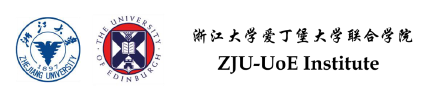
\includegraphics[scale=.5]{instituteLogo.png}}
\date{}

\begin{document}

\newtcolorbox{codebox}{enhanced,
    top=2pt,
    left=2pt,
    right=2pt,
    bottom=2pt,
    boxrule=0pt,
    leftrule=5pt,
    sharp corners,
    colback=gray!20,
    colframe=blue!60!black}

\begin{frame}
    \titlepage
\end{frame}

\begin{frame}
    {Plan for the next weeks}
    \begin{itemize}
        \item Week 8 - Traditional ML approaches in image analysis
        \item Week 9 - Convolutional neural networks (CNN)
        \item Week 10 - CNN architectures
        \item Week 11 - Practical aspects of using CNNs.
    \end{itemize}
\end{frame}

\begin{frame}
    {Learning objectives}
    \begin{columns}
        \begin{column}{0.8\textwidth}
            \begin{itemize}
                \item Describe use cases for machine learning in image analysis
                \item Describe the different types of machine learning algorithms
                \item Use Python to implement supervised and unsupervised ML algorithms for image analysis
            \end{itemize}
        \end{column}
        \begin{column}{0.2\textwidth}
            
\includegraphics[angle=-30, origin=tr, width=1.5\textwidth]{lightbulb.png}
        \end{column}
    \end{columns}
\end{frame}

\section{Introduction}

\begin{frame}
    {How can machine learning help?}
    \begin{columns}
        \begin{column}{.4\textwidth}
            Some example tasks that can be solved through ML
            \begin{itemize}[<+->]
                \item Classification of images
                \item Classification of pixels (segmentation)
                \item "Prediction" of images
            \end{itemize}
        \end{column}
        \begin{column}{.6\textwidth}
            \only<1>{
                \centering
                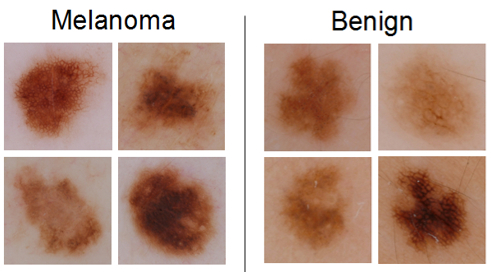
\includegraphics[width=.7\textwidth]{ISIC_melanoma.jpg}

                \footnotesize
                \raggedright
                ISIC melanoma classification competition.
                Many different solutions, including neural networks, support vector machines, deep learning\dots
            }
            \only<2>{
                \centering
                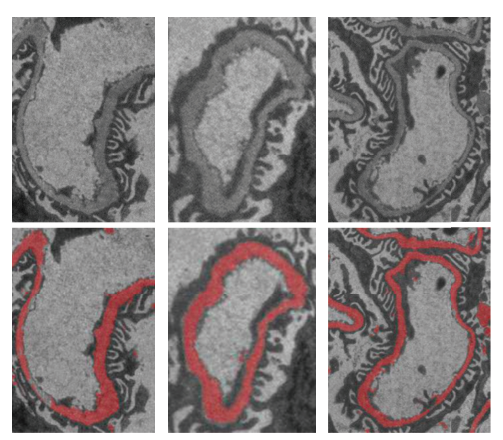
\includegraphics[width=.7\textwidth]{Cao2019_GBM.png}

                \footnotesize
                \raggedright
                Cao et al. 2019, Classification of glomerular basament membrane using Random Forests.
            }
            \only<3>{
                \centering
                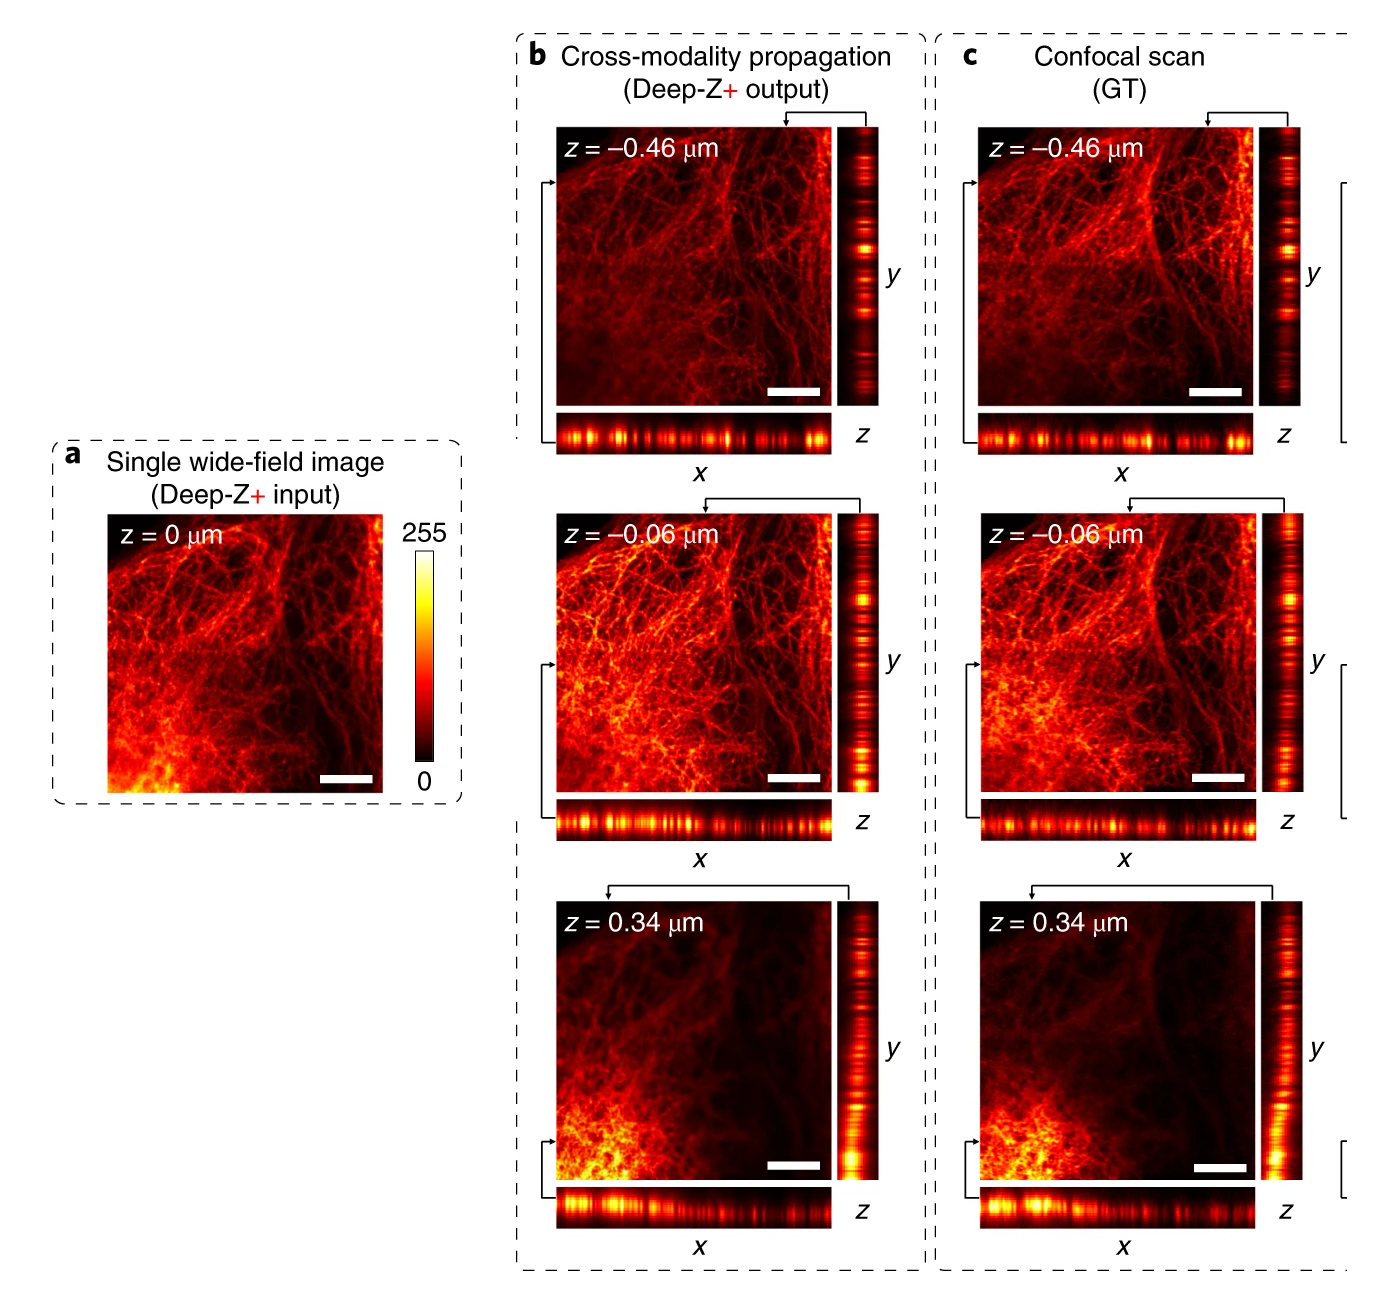
\includegraphics[height=.75\textheight]{deepz.jpg}

                \footnotesize
                \raggedright
                Wu et al., 2019 - Three-dimensional virtual refocusing of fluorescence microscopy images using deep learning

            }

        \end{column}
    \end{columns}
\end{frame}

\begin{frame}
    {The general process}
    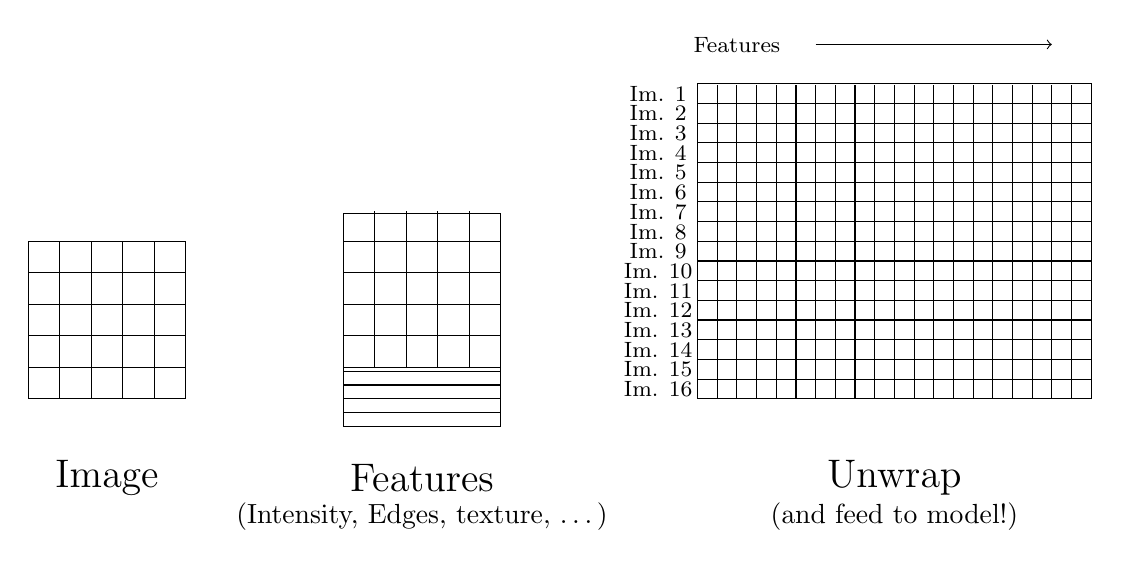
\begin{tikzpicture}
        \node at(1, -1) {\Large Image};
        \draw [fill=white] (0, 0) rectangle (2, 2);
        \draw [step=0.4] (0.01, 0.01) grid (1.99, 1.99);

        % Features
        \node at (5, -1) {\Large Features};
        \node at (5, -1.5) {\normalsize (Intensity, Edges, texture, \dots)};

        \foreach \y in {-10, -5, ..., 10}
        \draw [fill=white, yshift=\y] (4, 0) rectangle (6, 2);
        \draw [step=0.4] (4.01, 0.39) grid (5.99, 2.38);

        % Unwrap
        \draw (8.5, 0) rectangle (13.5, 4);
        \draw [step=0.25] (8.51, 0.01) grid (13.51, 3.99);

        \node at (11, -1) {\Large Unwrap};
        \node at (11, -1.5) {\normalsize (and feed to model!)};

        \foreach \i [count=\n] in {3.875, 3.625, ..., 0}
        \node at (8, \i) {\footnotesize Im. \n};
        \node at (9, 4.5) {\footnotesize Features};
        \draw [->] (10, 4.5) -- (13, 4.5);
    \end{tikzpicture}
\end{frame}

\begin{frame}
    {Supervised vs unsupervised ML}
    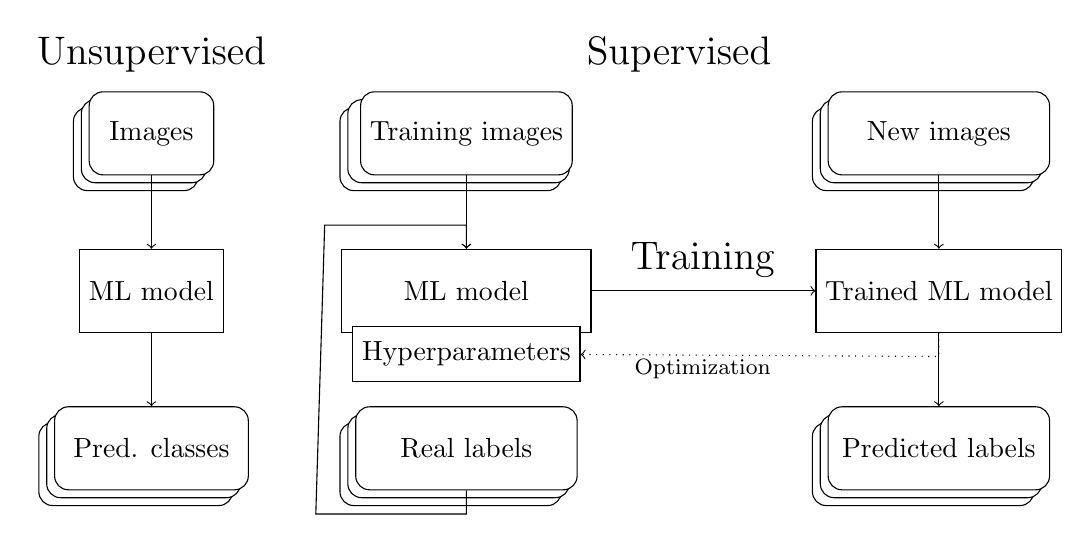
\begin{tikzpicture}
        \node at(0, 1) {\Large Unsupervised};

        \node[draw, rectangle, rounded corners=5pt, minimum height=3em, minimum width = 4.5em, fill=white] at (-0.2,-0.2) {};
        \node[draw, rectangle, rounded corners=5pt, minimum height=3em, minimum width = 4.5em, fill=white] at (-0.1,-0.1) {};
        \node[draw, rectangle, rounded corners=5pt, minimum height=3em, minimum width = 4.5em, fill=white] (img) at (0,0) {Images};
        \node[draw, rectangle, fill=white, minimum height=3em] (model2) at (0,-2) {ML model};

        \node[draw, rectangle, rounded corners=5pt, minimum height=3em, minimum width = 7em, fill=white] at (-0.2,-4.2) {};
        \node[draw, rectangle, rounded corners=5pt, minimum height=3em, minimum width = 7em, fill=white] at (-0.1,-4.1) {};
        \node[draw, rectangle, rounded corners=5pt, minimum height=3em, minimum width = 7em, fill=white] (classes) at (0,-4) {Pred. classes};

        \draw [->] (img) -- (model2);
        \draw [->] (model2) -- (classes);

        \pause
        \node at(6.7, 1) {\Large Supervised};

        \node[draw, rectangle, rounded corners=5pt, minimum height=3em, minimum width = 8em, fill=white] at (3.8,-0.2) {};
        \node[draw, rectangle, rounded corners=5pt, minimum height=3em, minimum width = 8em, fill=white] at (3.9,-.1) {};
        \node[draw, rectangle, rounded corners=5pt, minimum height=3em, fill=white] (train) at (4,0) {Training images};

        \node[draw, rectangle, rounded corners=5pt, minimum height=3em, minimum width = 8em, fill=white] at (3.8,-4.2) {};
        \node[draw, rectangle, rounded corners=5pt, minimum height=3em, minimum width = 8em, fill=white] at (3.9,-4.1) {};
        \node[draw, rectangle, rounded corners=5pt, minimum height=3em, minimum width = 8em, fill=white] (labels) at (4,-4) {Real labels};

        \pause

        \node[draw, rectangle, fill=white, minimum height=3em, minimum width = 9em] (model) at (4,-2) {ML model};
        \node[draw, rectangle, fill=white, minimum height=2em] (hyperparam) at (4,-2.8) {Hyperparameters};

        \node at (7, -1.6) {\Large Training};
        \node[draw, rectangle, fill=white, minimum height=3em] (modeltrained) at (10,-2) {Trained ML model};

        \draw [->] (train) -- (model);
        \draw [->] (labels) |-([shift={(-5mm,-3mm)}]labels.south west)-- ([shift={(-18mm,3mm)}]model.north)-| (model);
        \draw [->] (model) -- (modeltrained);
        \draw [->, dotted] (modeltrained) |-([shift={(0,-3mm)}]modeltrained.south)-- (hyperparam);
        \node at (7, -3) {\footnotesize Optimization};

        \pause

        \node[draw, rectangle, rounded corners=5pt, minimum height=3em, minimum width = 8em, fill=white] at (9.8,-0.2) {};
        \node[draw, rectangle, rounded corners=5pt, minimum height=3em, minimum width = 8em, fill=white] at (9.9,-0.1) {};
        \node[draw, rectangle, rounded corners=5pt, minimum height=3em, minimum width = 8em, fill=white] (newim) at (10,0) {New images};

        \node[draw, rectangle, rounded corners=5pt, minimum height=3em, minimum width = 8em, fill=white] at (9.8,-4.2) {};
        \node[draw, rectangle, rounded corners=5pt, minimum height=3em, minimum width = 8em, fill=white] at (9.9,-4.1) {};
        \node[draw, rectangle, rounded corners=5pt, minimum height=3em, minimum width = 8em, fill=white] (pred) at (10,-4) {Predicted labels};

        \draw [->] (newim) -- (modeltrained);
        \draw [->] (modeltrained) -- (pred);
    \end{tikzpicture}
\end{frame}

\section {Unsupervised methods}

\begin{frame}
    {Unsupervised learning}
    Examples of unsupervised learning include clustering methods (e.g. k-means) often combined with dimensionality reduction (PCA, UMAP).

    \only<2>{
        \centering
        k-means for segmentation (see Lecture 7)

        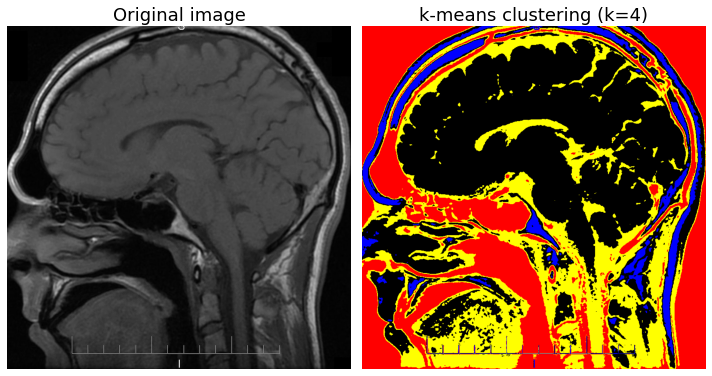
\includegraphics[width=.5\textwidth]{kmeans_MRI.png}
    }

    \only<3>{
        \centering
        \begin{columns}
            \begin{column}{.5\textwidth}
                \centering
                t-SNE clustering of images

                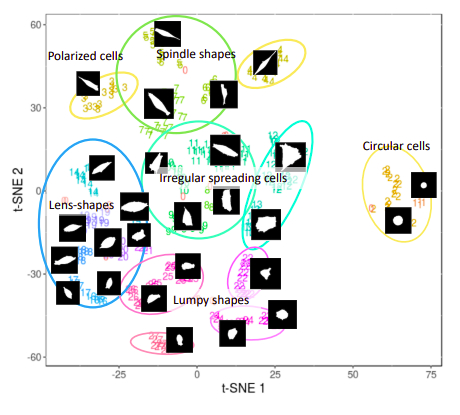
\includegraphics[width=.9\textwidth]{Bhaskar_2019_tsne_cell_shape.jpg}

                \footnotesize
                Bhaskar et al, 2019
            \end{column}
            \begin{column}{.5\textwidth}
                Dimensionality reduction methods map $Y = f(x_1, x_2, ..., x_n)$ to $Y = f(DR_1, ..., DR_m)$ with $m \leq n$. 
                
                They include linear transformations, such as PCA (principal component analysis), and nonlinear transformations, such as t-SNE (t-distributed stochastic neighbor embedding) or UMAP (uniform manifold approximation).
            \end{column}
        \end{columns}
    }

\end{frame}

\begin{frame}
    {A simple example...}
    Let's use t-SNE to classify handwritten digits!

    We are going to use the UCI digits dataset, by E. Alpaydin and C. Kaynak, containing 1797 8x8 images of handwritten digits from 0 to 9.

    It's a simple yet large dataset useful for quick image analysis tests!

    \centering
    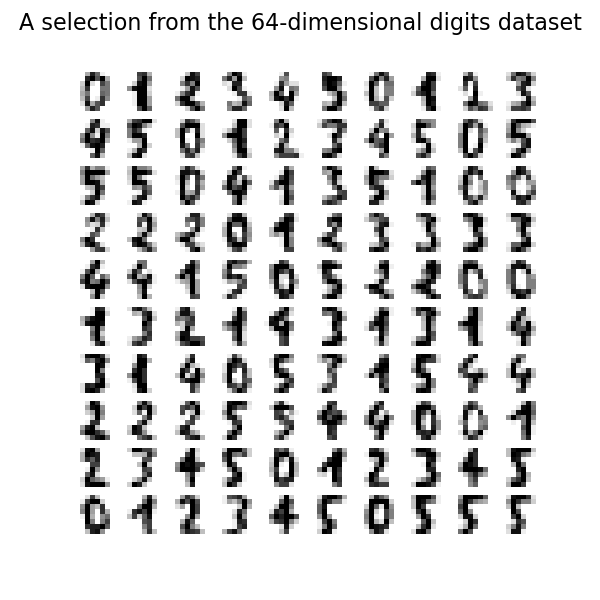
\includegraphics[width=.4\textwidth, trim=0 0 0 30, clip]{uci.png}
\end{frame}

\section {Supervised methods}

\begin{frame}
    {Supervised learning}
    Many different supervised learning algorithms have been used for image analysis.

    Commonly used:

    \begin{itemize}
        \item Logistic regression
        \item Support vector machines (SVM)
        \item Random forests (RF)
        \item Neural networks (Lecture 11)
        \item Convolutional neural networks (Lectures 12 and beyond)
    \end{itemize}
\end{frame}

\begin{frame}
    {Supervised learning algorithms - Logistic regression}
    \centering
    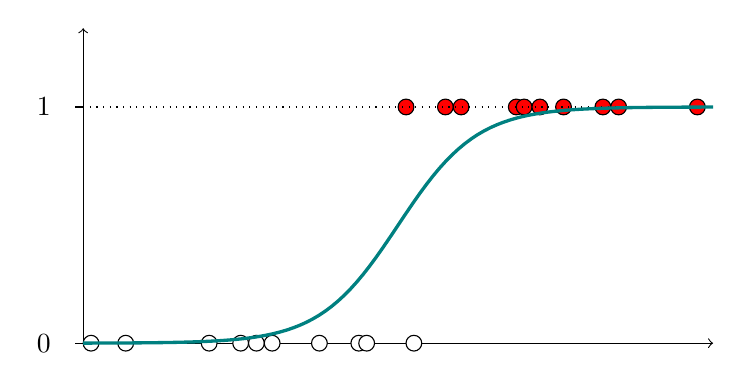
\begin{tikzpicture}
        % axis with ticks
        \draw [<->] (0, 4) -- (0, 0) -- (8, 0);
        \draw (0, 3) -- (-0.1, 3);
        \draw (0, 0) -- (-0.1, 0);
        \node at (-0.5, 0) {0};
        \node at (-0.5, 3) {1};

        % points on 0
        \foreach \x in {0.1, 0.54, 1.6, 2, 2.2, 2.4, 3, 3.5, 3.6, 4.2}
        \draw [fill=white] (\x, 0) circle (0.1);
        % points on 1
        \foreach \x in {4.1, 4.6, 4.8, 5.5, 5.6, 5.8, 6.1, 6.6, 6.8, 7.8}
        \draw [fill=red] (\x, 3) circle (0.1);

        \draw [thin, dotted] (0, 3) -- (8, 3);
        % logistic regression
        \draw [very thick, teal, domain=0:8,samples=100] plot (\x,{3/(1+(exp(-2*(\x-4)))});
    \end{tikzpicture}

    Logistic regression is a simple supervised learning algorithm that is used to predict the class of a given data point. 
    
    It is mostly used to predict binary outcomes but can be extended to multi-class classification (multinomial logistic regression).
\end{frame}

\begin{frame}
    {Supervised learning algorithms - support vector machines}
    \centering
    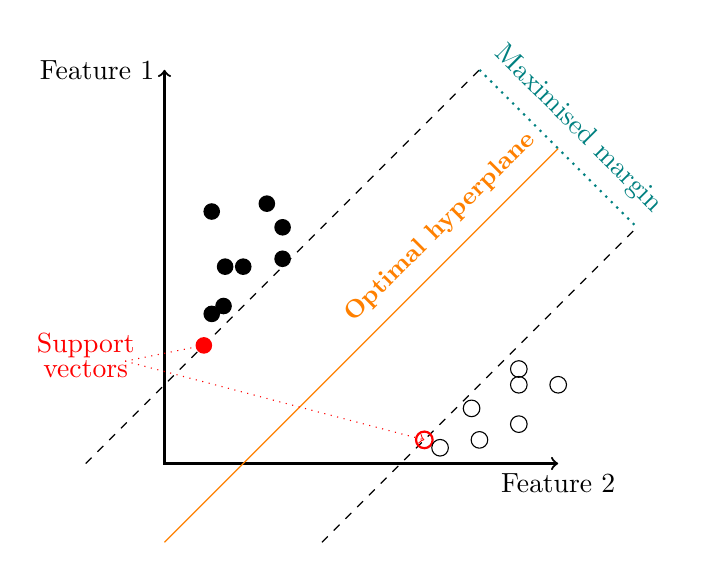
\begin{tikzpicture}
        % Draw axes
        \draw [<->,thick] (0,5) node (yaxis) [left] {Feature 1}
        |- (5,0) node (xaxis) [below] {Feature 2};
        % draw line
        \draw [color=orange] (0,-1) -- (5,4); % y=x-1
        \draw[dashed] (-1,0) -- (4,5); % y=x+1
        \draw[dashed] (2,-1) -- (6,3); % y=x-3
        % \draw labels
        \draw (3.5,3) node[color=orange, rotate=45,font=\small]
        {\textbf{Optimal hyperplane}};
        % draw distance
        \draw[dotted, thick, color=teal] (4,5) -- (6,3);
        \draw (5.25,4.25) node[color=teal, rotate=-45] {Maximised margin};
        % draw negative dots
        \node [color=red] at (-1, 1.5) {Support};
        \node [color=red] at (-1, 1.2) {vectors};
        \draw [->, color=red, thin, dotted] (-0.5, 1.3) -- (0.5, 1.5);
        \draw [->, color=red, thin, dotted] (-0.5, 1.3) -- (3.3, 0.3);
        \fill[red] (0.5,1.5) circle (3pt);
        \fill[black] (1.5,2.6) circle (3pt);
        \fill[black] (1,2.5) circle (3pt);
        \fill[black] (0.75,2) circle (3pt);
        \fill[black] (0.6,1.9) circle (3pt);
        \fill[black] (0.77, 2.5) circle (3pt);
        \fill[black] (1.5,3) circle (3pt);
        \fill[black] (1.3,3.3) circle (3pt);
        \fill[black] (0.6,3.2) circle (3pt);
        % draw positive dots
        \draw[red,thick] (3.3,.3)  circle (3pt);
        \draw[black] (4.5,1) circle (3pt);
        \draw[black] (4.5,1.2) circle (3pt);
        \draw[black] (4.5,.5) circle (3pt);
        \draw[black] (3.9,.7) circle (3pt);
        \draw[black] (5,1) circle (3pt);
        \draw[black] (3.5,.2) circle (3pt);
        \draw[black] (4,.3) circle (3pt);
    \end{tikzpicture}

    A support vector machine (SVM) uses a linear decision boundary to classify data points. It determines the optimal hyperplane that separates the data points into two classes.
\end{frame}

\begin{frame}
    {Random forest}

    \centering
    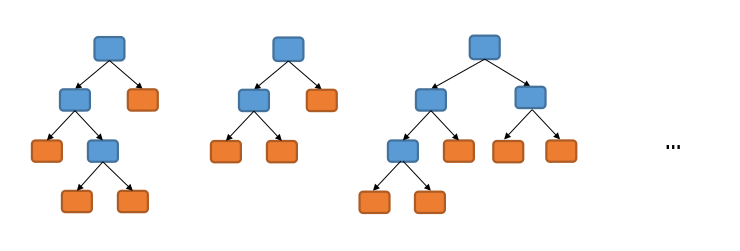
\includegraphics[width=\textwidth]{RandomForest.png}

    Random forest is an ensemble method for classification and regression.

    It classifies samples using many binary trees, fitted on various sub-samples of the dataset. A majority votes from these trees decides the outcome. This improves prediction accuracy and controls over-fitting.
\end{frame}

\begin{frame}
{The bias-variance tradeoff}
We want to train our model to perform some task. However, just like any statistical model, we don't want to \textbf{overfit}.

\only<1-2>{\centering
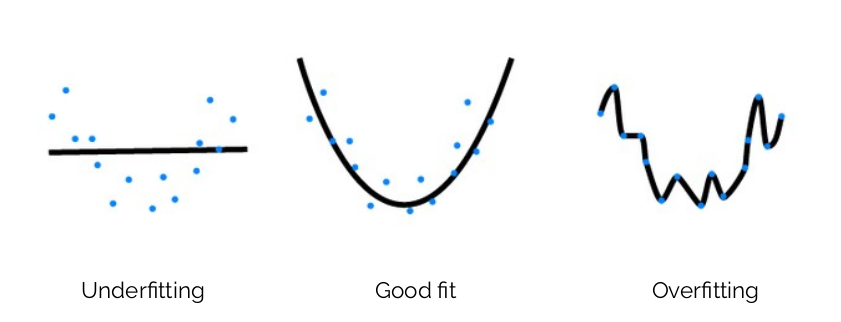
\includegraphics[width=.6\textwidth]{fitting.png}

\raggedright
In ML, we often describe this in terms of \textbf{bias} and \textbf{variance} errors.
\pause
\begin{itemize}
\item \textbf{Bias} derives from erroneous assumptions in the learning algorithm. High bias can cause an algorithm to miss the relevant relations between features and target outputs (underfitting).
\item \textbf{Variance} derives from sensitivity to small fluctuations in the training set. High variance may result from an algorithm modeling the random noise in the training data (overfitting).
\end{itemize}
\footnotesize(Adapted from Wikipedia)
}
\only<3>{
\centering
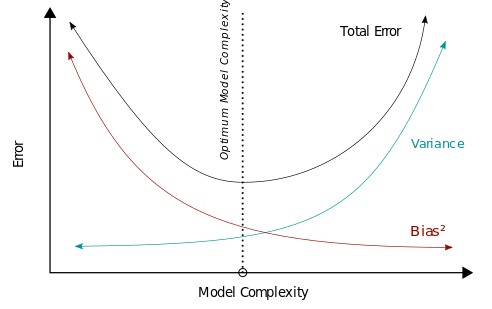
\includegraphics[width=.8\textwidth]{Bias_variance.jpg}
}
\end{frame}
\begin{frame}
    {Data splitting}
    In order to avoid overfitting we can split our dataset in three parts:

    \begin{itemize}
        \item \textbf{Training set} - used to train the model
        \item \textbf{Validation set} - used to estimate model performance during training or while tuning the model hyperparameters. Especially important for neural network.
        \item \textbf{Test set} - used to test the trained model
    \end{itemize}

    \centering
    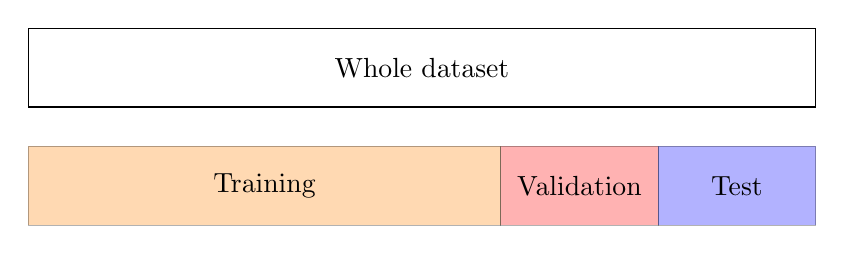
\begin{tikzpicture}
        \draw [fill=white] (0, 2.5) rectangle (10, 3.5);
        \node at (5, 3) {Whole dataset};
        \draw [fill=orange, opacity=0.3] (0, 1) rectangle (6, 2);
        \node[align=center] at (3, 1.5) {Training};
        \draw [fill=red, opacity=0.3] (6, 1) rectangle (8, 2);
        \node at (7, 1.5) {Validation};
        \draw [fill=blue, opacity=0.3] (8, 1) rectangle (10, 2);
        \node at (9, 1.5) {Test};
    \end{tikzpicture}
\end{frame}

\begin{frame}
    {The training process}
    \centering
    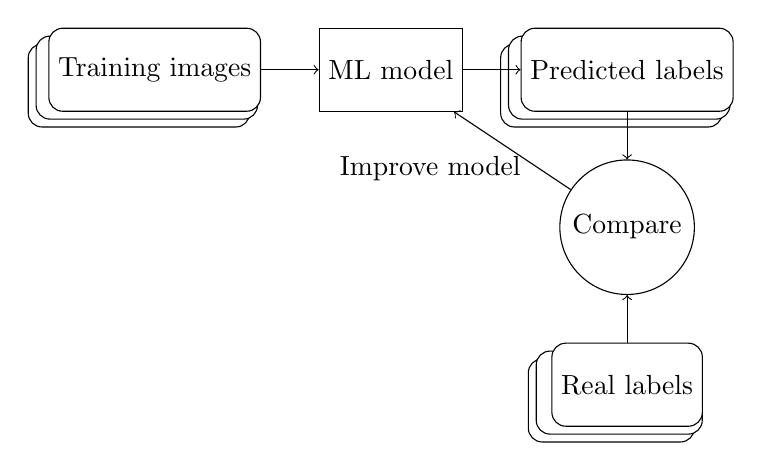
\begin{tikzpicture}
        \node[draw, rectangle, rounded corners=5pt, minimum height=3em, minimum width = 8em, fill=white] at (-0.2,-0.2) {};
        \node[draw, rectangle, rounded corners=5pt, minimum height=3em, minimum width = 8em, fill=white] at (-0.1,-.1) {};
        \node[draw, rectangle, rounded corners=5pt, minimum height=3em, fill=white] (train) at (0,0) {Training images};
        \node[draw, fill=white, rectangle, minimum height=3em] (model) at (3,0) {ML model};
        \node[draw, rectangle, rounded corners=5pt, minimum height=3em, minimum width = 8em, fill=white] at (5.8,-0.2) {};
        \node[draw, rectangle, rounded corners=5pt, minimum height=3em, minimum width = 8em, fill=white] at (5.9,-0.1) {};
        \node[draw, rectangle, rounded corners=5pt, minimum height=3em, fill=white] (pred) at (6,0) {Predicted labels};

        \node[draw, rectangle, rounded corners=5pt, minimum height=3em, fill=white, minimum width = 6em] at (5.8,-4.2) {};
        \node[draw, rectangle, rounded corners=5pt, minimum height=3em, fill=white, minimum width = 6em] at (5.9,-4.1) {};
        \node[draw, rectangle, rounded corners=5pt, minimum height=3em, fill=white] (GT) at (6,-4) {Real labels};
        \node[draw, circle, fill=white, minimum height=1.5em] (comp) at (6,-2) {Compare};
        \node at (3.5, -1.25) {Improve model};

        \draw [->] (train) -- (model);
        \draw [->] (model) -- (pred);
        \draw [->] (pred) -- (comp);
        \draw [->] (GT) -- (comp);
        \draw [->] (comp) -- (model);
    \end{tikzpicture}

    We will explore this more in details in the upcoming lectures!
\end{frame}

\begin{frame}
{Supervised learning handwritten digits}
We will use the handwritten digits dataset again, but this time we will train a supervised model (SVM) to predict the class of the digit.

\centering
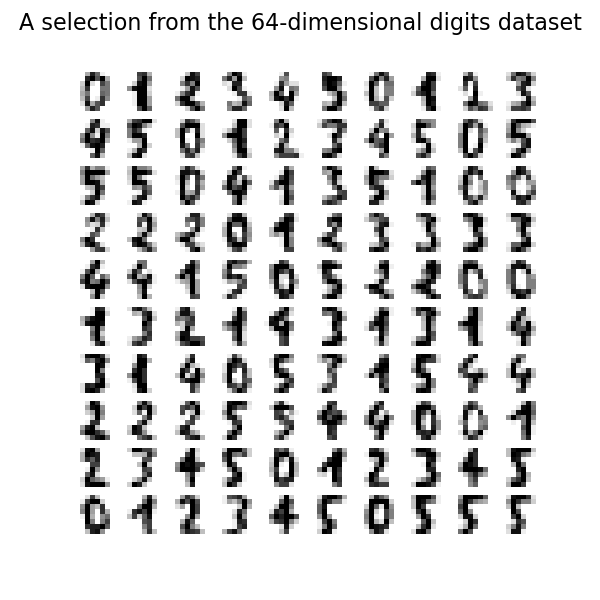
\includegraphics[width=.4\textwidth]{uci.png}
\end{frame}
\end{document}

